%TEX root = ../dissertation.tex

\chapter{Proposed Solution}
\label{chapter:proposed_solution}

Before attempting to develop a protocol, or solution, that meets our goals and properly addresses the problems and attacks described in the previous chapters, it is important to define the scope of our work. A common appropriate way to do so is by presenting both a scenario and architecture of the solution. The Internet of Things is currently a hot trend and this work could potentially apply and benefit a wide spectrum of applications, ranging from home environments to large enterprise networks. However, these are domains that have different requirements. A home application should be easy to setup and not require complex configurations to the user. An enterprise solution can benefit from additional administrative configurations as long as the deployment of the devices can be done quickly and easily due to their potential large number. Our work will position itself in the middle of these two domains. We are looking at a complexity and number of devices greater than a home environment but it is not our focus to provide solutions for enterprise networks and their deployment restrictions. It is our belief that a Smart University Campus is an adequate scenario and can effectively demonstrate the needs targeted by our work. In the following sections we will apply the information gathered in the related work sections to formally define what we are trying to achieve, what are the difficulties in achieving those goals and how can we overcome them. Then, a model of a campus with the proposed energy-efficient network architecture will be presented and their component roles explained. Finally, we will discuss additional improvements that are currently out of the scope of this work but can be left for future work.

\subsection{Objectives and Requirements}
\paragraph{}
One of the major concerns regarding \gls{IoT} application is the communication model. For our work, we pose as requirement that the system is power-aware and uses the minimum energy possible. Additionally, the following set of objectives is desirable to build trust and allow secure communications to take place.

\begin{itemize}
	\item Confidentiality: Without confidential message transmission, packets would flow in the network in plain text. Attackers could sniff the packets in order to obtain information, and depending on the application, this could be a security breach. Even if there is no critical data being sent, privacy is still compromised.\\
	\item Integrity: Assuring message integrity means that the message was not modified between the source and its destination. Without integrity we could not rely on the received data since it could have been, intentionally or not, modified on the fly, and be providing the system wrong information.\\
	\item Authentication: The studied type of networks relies on hop-to-hop communication, meaning several nodes will take place in forwarding a packet. If they are not authenticated they could perform a wide range of attacks and disrupt the network.
\end{itemize}

\subsection{System Architecture and Message Flow}
\paragraph{}

As stated in the beginning of the chapter, we will use a Smart Campus scenario. Being aware of the technological improvements on sensor networks and building management technologies, the \gls{IST} administration decided to improve the monitoring the overall conditions of the buildings and inside environments in order to better preserve its assets. To cope with the new requirements, we propose a solution for the monitoring of the campus sections by deploying a wireless sensor network on each building, connected to a central management station operated by the available staff. The scenario will be based on the \gls{IST} campus model. An overview of the system and its components over the \gls{IST} blueprints can be found in Figure \ref{fig:global_architecture}. Regarding each individual component:

\begin{itemize}
	\item Numeric Nodes: Represent the network sensor nodes, the most constrained element of the network. They cooperate to build the topology and route messages hop-by-hop until the root is reached. These are fully equipped with the energy efficient protocol stack defined in Section 4.1\\
	\item Alphabetical Nodes: Represent the root node of each section network topology. They are equipped with the same stack of the numbered nodes but are more powerful, preferentially not battery powered and act as the bridge between the constrained 6LoWPAN environment and the central management station. These nodes must be more powerful than the numeric ones so that they can process all the requests between a group of sensors and the management station. Also, although the numeric nodes use low-power wireless radios, the alphabetical nodes must be capable of interfacing with more power hungry radios and protocols therefore requiring more resources. This differentiation allows numeric nodes (the large portion of the network devices) to keep their very constrained nature, consuming less energy, an still be able to communicate with external devices.\\
	\item Management Station: A black box model of the core components of the system. Each building reports to the central station and the staff monitors the status through it. A white box model will be shown in the following sections.\\
	\item Client: The system's clients can be any user with access credentials, but mostly the staff members. They can access the management station either from within the local network or from outside through the Internet.\\
\end{itemize}
 
\begin{figure}[h]
  \centering
  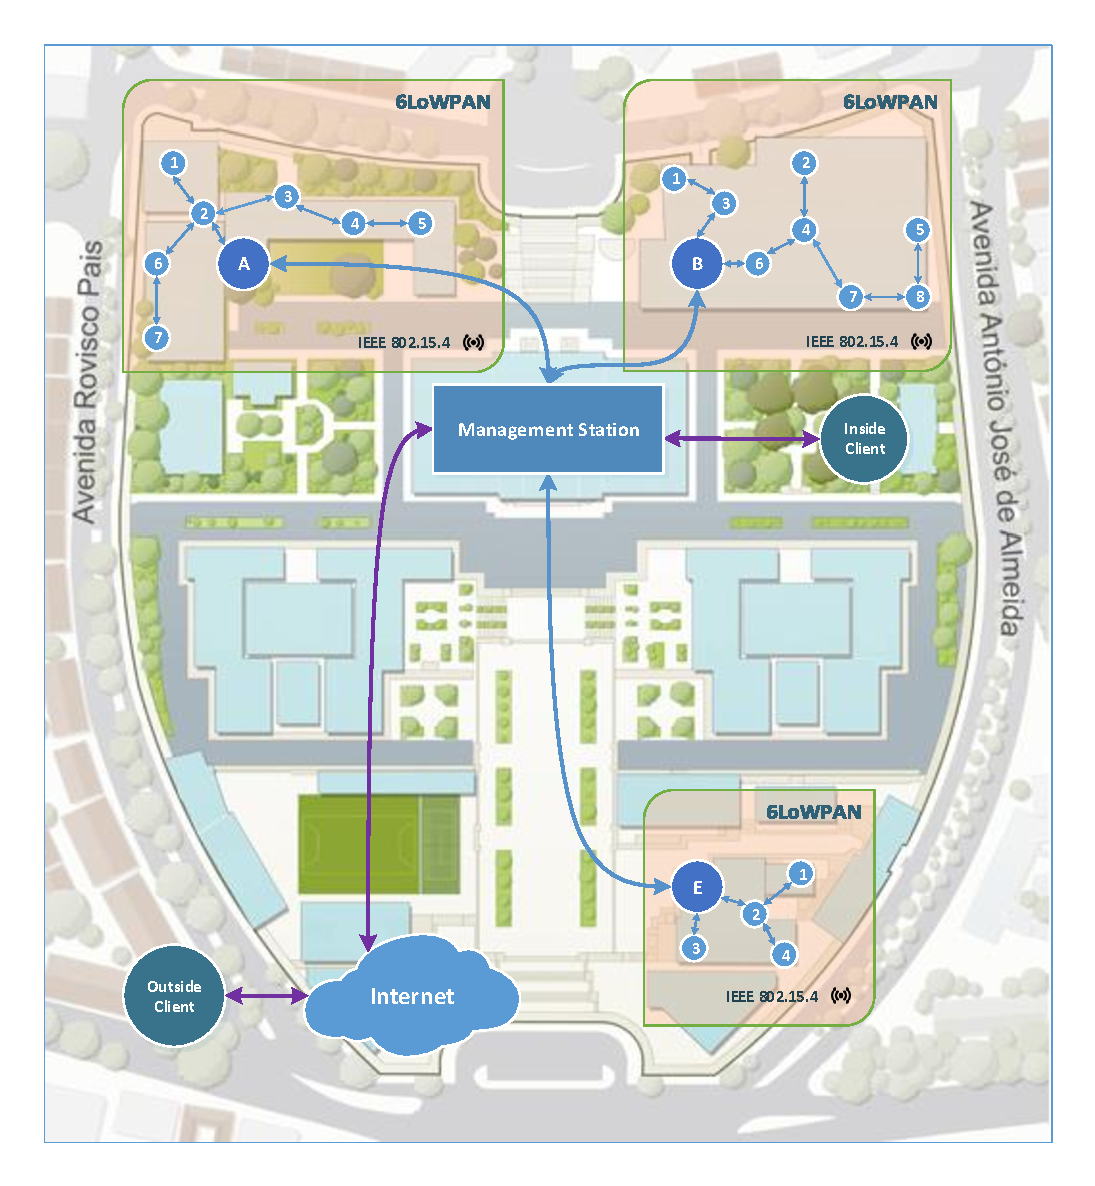
\includegraphics[width=0.9\linewidth]{figures/Global_Architecture.pdf}
  \caption{Global System Architecture}
  \label{fig:global_architecture}
\end{figure}

\paragraph{\textbf{Central Management Station}}
\paragraph{}

The central management station is divided in five main components. A white box schematic of the core components and interactions can be found in Figure \ref{fig:core_components}. Regarding each individual component:

\begin{itemize}
	\item Key Store: This component is responsible for storing the shared network key for the RPL protocol and a mapping between each network device and its key pair. This information is facilitated to the Client Observer for creating a secure connection to each sensor node;\\
	\item Bootstrapper: The bootstrapper acts as the interface between the management station and the network devices. It generates the device key pair and writes it together with the shared network key and the Client Observer public key into the new device;\\
	\item CoAP Client Observer:  The one and only client in the network. Instead of the user directly requesting the sensor readings, the client will observe each resource and be notified of the new value. Each time it receives an update, it stores the information on the Data Server for the clients to use;\\
	\item Data Server: A database with mappings of each node to the most up to date value reported. It's updated by the client observer and used on demand by the clients;\\
	\item Proxy: Responsible for bridging requests coming from the Internet to the Data Server. Responsible for authenticating the external clients and providing access to the Data Server information.\\
\end{itemize}

Although each user could access the system through a \gls{CoAP} terminal and request the most up-to-date readings from the sensor nodes, this approach would cause many overheads in the system. Firstly, and since many clients can connect from different locations, many requests would be performed to the sensor nodes for the same information. Additionally each sensor node would need to be pre-installed with the public keys of all the different user terminals. This would mean additional memory usage in the physical devices, and more requests to the already constrained battery operated network. With the single client approach acting as an observer, only one message needs to go through the network for each new reading.

\begin{figure}[h]
  \centering
  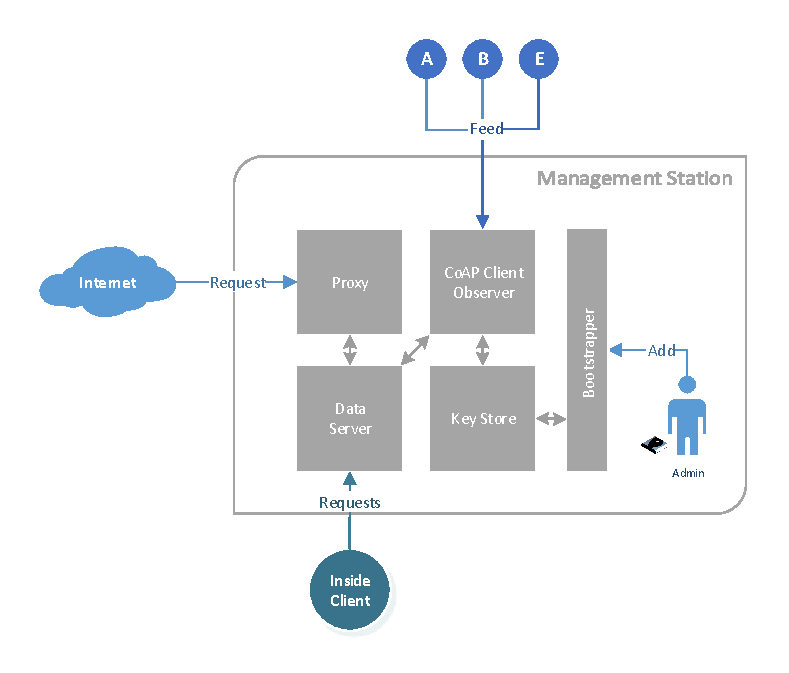
\includegraphics[width=0.92\linewidth]{figures/White_Box_Model.pdf}
  \caption{Central Management Station}
  \label{fig:core_components}
\end{figure}

\paragraph{\textbf{Credentials Configuration}}
\paragraph{}

In order to achieve secure communications, the new node must connect to the RPL network in a secure way, that is by using a pre-shared group key. After that network setup, it will also need to make a DTLS handshake with the client observer, for that needing a key pair and the public key of the client observer. That information is written into the device during the configuration phase, done by the staff members. Figure \ref{fig:sequence_bootstrapping} shows a sequence diagram of the initial configuration phase. This process will be fully automated without requiring the staff administrator any knowledge of the inner workings of the network and authentication procedures.

\begin{figure}[h]
  \centering
  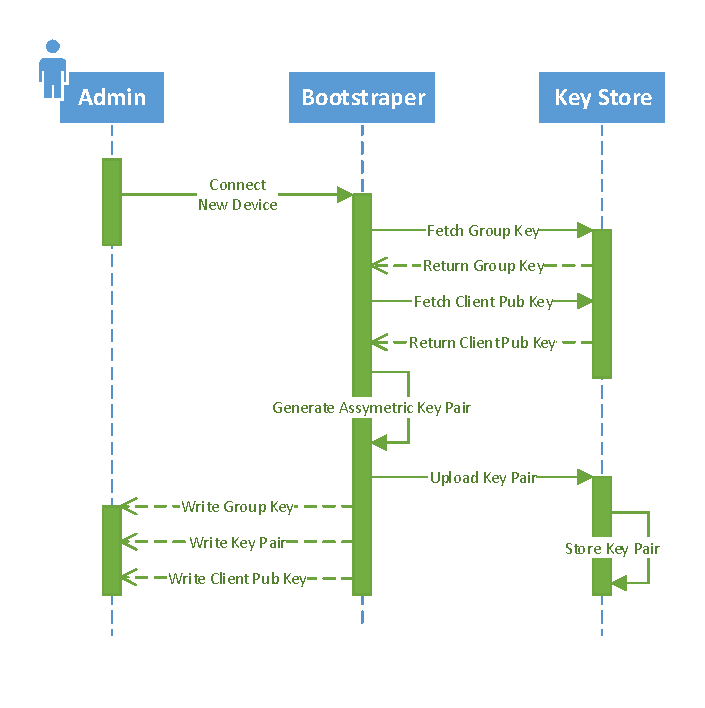
\includegraphics[width=0.8\linewidth]{figures/Sequence_Bootstrapping.pdf}
  \caption{New Device Initial Configuration}
  \label{fig:sequence_bootstrapping}
\end{figure}

As shown in the sequence diagram, the process is initiated by a staff member by connecting a new device to the bootstrapper. The bootstrapper automatically requests the network group key from the key store and the Client Observer public key. Then a new key pair is generated and stored in the key store for that device. Finally the bootstrapper writes the group key, the key pair and the Client Observer public key into the device.
\pagebreak
\paragraph{\textbf{Network Layer Bootstrapping}}
\paragraph{}

After the credentials configuration phase, the new device is fully equipped with the security credentials required for joining the RPL network. Figure \ref{fig:sequence_network_admission} shows a sequence diagram of process started by the new node to join the network topology. The vocabulary used to represent the message exchange was previously presented in Section \ref{sec:network_layer}. All the message exchange is done with the secure versions of the RPL control messages, meaning the data is cyphered with the shared group key.

\begin{figure}[h]
  \centering
  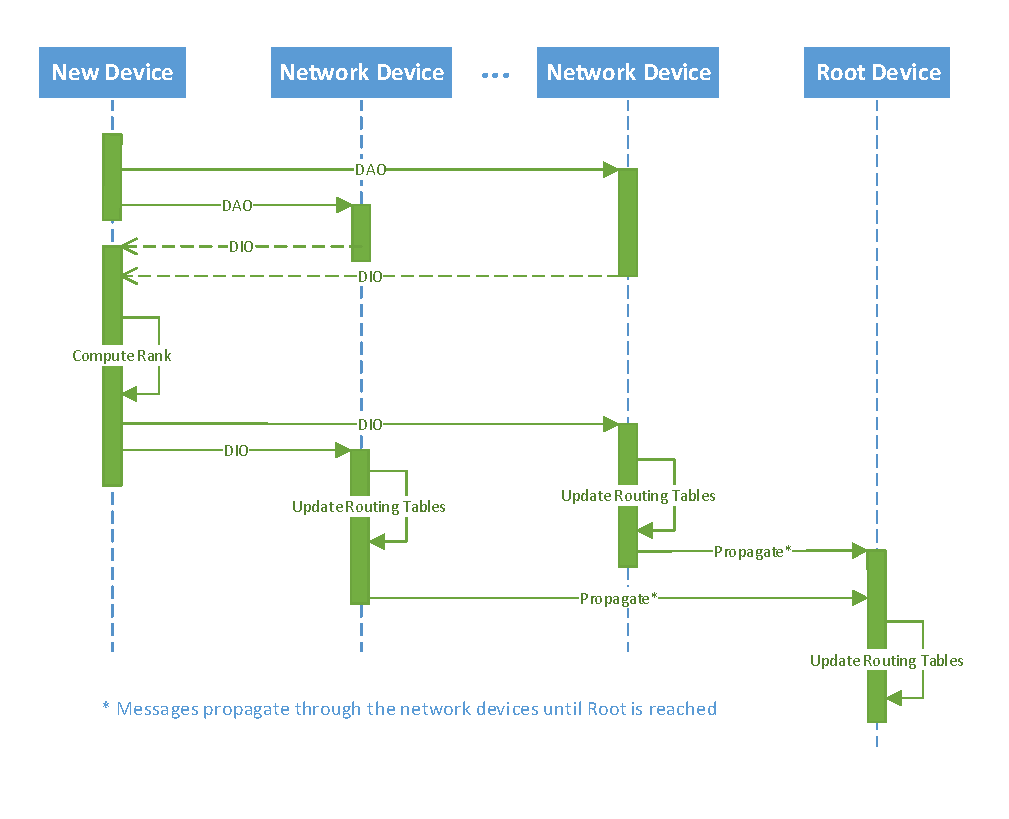
\includegraphics[width=0.95\linewidth]{figures/Sequence_Network_Admission.pdf}
  \caption{Network Layer Bootstrapping}
  \label{fig:sequence_network_admission}
\end{figure}

As shown in the sequence diagram, the process is initiated by the joining device by broadcasting \gls{DAO} messages to any available neighbour devices in range. The receiving nodes will reply to the new device with a \gls{DIO} message that provides graph routing information. With this information the new device is able to compute its rank (the distance towards the root) and define its parents based on that metric. After that process is complete, the new device tells his neighbours about its position in the graph using a \gls{DIO} message and the receiving nodes update their routing tables so that downwards traffic can now reach the new node. This information is further propagated up the network topology until the root is reached.

\paragraph{\textbf{Application Layer Bootstrapping}}
\paragraph{}

Although the device is now bootstrapped at the network layer, it still needs to discover and be discovered at the application layer. This means contacting the Client Observer, securing the channel through \gls{DTLS} and then send new readings as they occur. Figure \ref{fig:sequence_application_admission} shows a sequence diagram of process started by the new node to join the \gls{CoAP} network.

\begin{figure}[h]
  \centering
  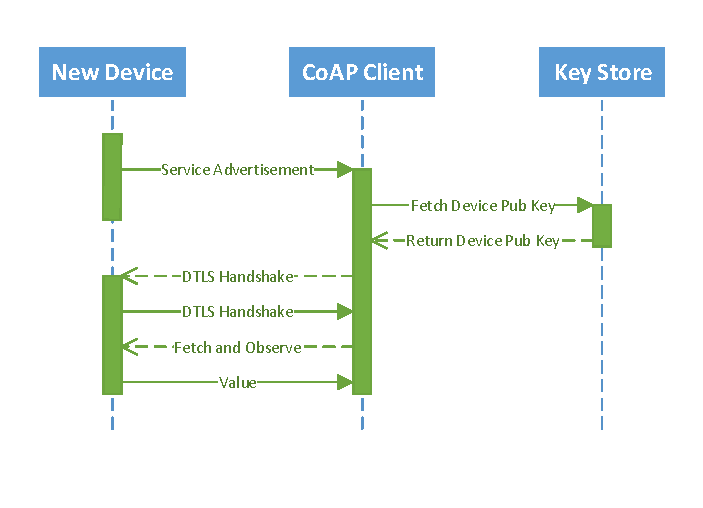
\includegraphics[width=0.8\linewidth]{figures/Sequence_Application_Admission.pdf}
  \caption{Application Layer Bootstrapping}
  \label{fig:sequence_application_admission}
\end{figure}

As shown in the sequence diagram the process is started by the new device that advertises its services to the network. That message is eventually received by the Client Observer who uses the new device public key, stored in the key store to start a \gls{DTLS} secured channel. After the handshake is completed, the Client Observer requests the latest readings to the sensor and sets the observe option meaning each time there is a change in the sensor reading the client will be notified.

\subsection{Limitations and Future Work}
\paragraph{}
The use of secure RPL messages with the pre-shared group key together with the raw public/private key pairs assures that a new device is properly authenticated when joining the network as well as confidentiality and integrity of the propagated packets. However, public key cryptography is based on computationally intensive mathematical functions that are not very efficient on constrained devices. In fact, asymmetric encryption techniques are almost 1000 times slower than symmetric techniques because they require more computational processing power \cite{Kumar2011}. In the event that our work reveals the impossibility to use public key cryptography on the most constrained sensing nodes, symmetric cryptography is hereby posed as an alternative.\\
Also, as discussed in Section \ref{sec:attack_analysis}, an attacker could try to introduce himself in the network by stealing the keys from a deployed device. The solutions for that attack can be either software based, assuring that secure memory areas cannot be copied to external locations. Or hardware based, certain integrated circuits assure the stored information cannot be read from them \cite{Lesjak2014}. This attack will not be mitigated in our system as we believe the mitigation strategies are outside the scope of this project and more related to other engineering fields of research.\\